\section{存在唯一性定理}

\subsection{什么是存在唯一性定理}
朱鹭子:在此之前,我们得到的ODE全都无视了它是否有没有解,\textbf{解是否唯一},这里倒是准备和你说一下这些。

琪露诺:存在性吗……感觉很枯燥……

\begin{tho}[label=czwy]{存在唯一性定理}{}
	对于一个将导数分离出来的ODE:
	\[
		\dx=f(t,x)
		.\]
	如果 \(f\)在开区域 \(\overline{\symcal{I} }\) 上面满足:任意 \(\overline{\symcal{I} }\)中的闭矩形区域 \(\overline{\symcal{G}} \)上都满足Lipschitz条件:
	\[
		\left\vert f(t,x_1)-f(t,x_2) \right\vert \leqslant L \left\vert x_1-x_2 \right\vert ,\,\forall (t,x_1),(t,x_2)\in \overline{\symcal{G}}
		.\]

	且有初始条件:\(x(t_0)=x_0\),则存在解 \(x=X(t) \)在点 \((t_0,x_0)\)的邻域内有定义,且该解可以延拓到任意接近 \(\overline{\symcal{I} }\)的边界。
\end{tho}

琪露诺:???????这都啥啊……

朱鹭子:这确实很怪……让我尝试说明一下。为了方便,我们先从单变量的实函数开始说明:
\[
	y=f(x) \,\mbox{\kaiti 或者}\, f: \overline{\symcal{I} } \subseteq\symbb{R}     \mapsto  \symbb{R}
	.\]
如果存在常数 \(L\)使得:
\[
	\left\vert f(a)-f(b) \right\vert \leqslant L \left\vert a-b \right\vert, \,\forall a,b\in  \overline{\symcal{I} }
	.\]

则我们称 \(f\)满足Lipschitz 条件,而 \(L_{\mathrm{m}in}\)被称为Lipschitz常数,如果这个常数小于一,我们会称 \(f\)是\textbf{压缩映射}。这个我们先不管了,你只要先知道,如果 \(f\) 是在区域内满足Lipschitz条件,那么给出 \(x\)的一个初值条件时候,\(x\)唯一可解。

另外一件事是,要确立一个函数的Lipschitz条件是非常麻烦的一件事,我们可以用:\(\dfrac{\uppartial f}{\uppartial x}
\)连续来替代。

琪露诺:看起来要好不少……至少有比较良好的方式了。

朱鹭子:对,现在你可以考虑以下这种,如果你没法把 \(x'\)分离出来怎么办?
\[
	F(x,x',t)=0
	.\]
这种呢?

琪露诺:啊……我感觉……可以试试隐函数存在定理,只要在邻域内 \(\dfrac{\uppartial F}{\uppartial x'}\Bigg|_{(t_0,x_0)}\neq 0\)的话,那我就可以在这里把 \(x'\) 解出来。

朱鹭子:没错,这意味着有一些\(\dfrac{\uppartial F}{\uppartial x'}\Bigg|_{(t_0,x_0)}=0\)的情况。
\subsection{包络线}

琪露诺:什么情况呢?

朱鹭子:我和你说个问题,如果有这样一种解,它的并不属于通解,但它也是微分方程的解,而且满足一种特殊的性质:
\begin{itemize}
	\item 这条曲线的每一点处都有一条通解曲线与其相切。
\end{itemize}
这种曲线被称为上述通解积分曲线族的\textbf{包络}。

琪露诺:包络?那是什么?

朱鹭子:在这里我可以给出一些例子:

\begin{center}
	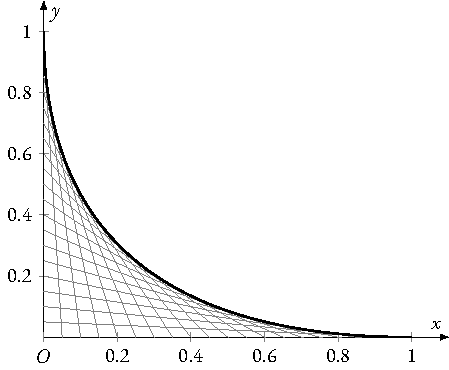
\includegraphics{envelope.pdf}
\end{center}

假如有这样一些直线,它的 \(y\)轴截距和 \(x\)轴截距加起来是 1,并且那两个截距都大于零,图中画出了一些这样的直线(灰色部分),那么黑色曲线就是它的包络线。

琪露诺:哇,好像它就是把灰色线的运动紧紧包裹住了一样。

朱鹭子:差不多,不过实际上应该是相切吧(笑),比如离原点距离为1的直线的包络就是单位圆嘛。

琪露诺:那包络线怎么求呢?

朱鹭子:实际上我们知道那些通解,或者更广泛地,曲线族的形式可以表示为:
\[
	F(t,x,c_1)=0
	.\]

那么包络线的方程是会满足:
\[
	\begin{cases}\\[-2em]
		F(t,x,c_1) =0, \\
		\dfrac{\uppartial F}{\uppartial c_1}=0.
	\end{cases}\tag{E}
\]

针对 \(c_1\)的参数方程。但是满足这方程的曲线可能有很多,其中并不一定有包络线。但毫无疑问的是,包络线的确是一种特殊的存在。现在我们来看看包络线和微分方程的关系:

想想看,对于一个一阶微分方程,它对解曲线的性质描述只精确到一阶导数,那么看看我们的包络线——每一点都有一条曲线族中的曲线\textbf{与之相切},如果这族曲线是一个一阶ODE的解的话……

琪露诺:那是不是意味着,这个包络上面所有点都满足那个方程……因为导数一样了, 点也在那些解的曲线上面。

朱鹭子:没错!这其实就是说这个包络线也是ODE的解,这其实是ODE的\textbf{奇解}。当然这也就意味着不满足那个唯一性条件了,所以根据你之前说的……

琪露诺:隐函数存在定理。

朱鹭子:对,所以对于初始条件 \(x(t_0)=x_0\),应当有:
\[
	\dfrac{\uppartial F(t,x,x')}{\uppartial x'}\Bigg|_{(t_0,x_0)}
	.\]

但这只是最基本的条件,事实上,由E式子我们知道,我们把 \(\dx\) 看成是 \(c_1\)……然后实际上这个\ruby[g]{包络}{奇解}应该满足:
\[
	\begin{cases}\\[-2em]
		F(t,x,x')=0 , \\
		\dfrac{\uppartial F}{\uppartial x'}=0.
	\end{cases}
\]

将这玩意把 \(x'\)消去就是包络线要满足的方程了,同理,这只是其中一个条件而已。

琪露诺:又来……全都是仅仅能满足的程度吗?有没有充要条件呢?

朱鹭子:饶了我吧,我暂时还不知道(笑),上面这个主要是来判断一个ODE有没有奇解的,这样的解往往会……就像幻想乡对于外界一样吧(笑)。

琪露诺:又是听不懂的比喻……

朱鹭子:这倒是有个出名的例子,叫做Clairaut微分方程:
\[
	x=t\dx+f\left( \dx \right)
	.\]

你试试鼓捣鼓捣这个ODE。

琪露诺:哦……首先两边对 \(t\)求导,得到:
\[
	\dx=x\symscr{D} ^2_t(x)+\dx+f'\left( \dx \right)\symscr{D} ^2_t(x)
	.\]

约去两边的 \(\dx\)得到:
\[
	\symscr{D} ^2_t(x)\left( x+f'\left( \dx \right)  \right) =0
	.\]

所以事实上是 \(\symscr{D} ^2_t(x)=0\implies \dx=c_1\)和 \(x+f'\left( \dx \right)=0 \)。

接下来我只需要积分就可以……哦直接代方程……就可以:
\[
	x=c_1x+f(c_1)
	.\]

哇是一坨子直线。所以你的意思是说另外一个 \(x+f'\left( \dx \right)=0\)其实是这些直线的包络吗?

朱鹭子:事实上的确是这样,在这里就先不验证了,但不管怎么样,记住有奇解存在这件事还是相当重要的。
